\documentclass{report}
\usepackage{ptext}
\usepackage{lipsum}
\usepackage{graphicx}
\usepackage{ptext}

\input{Boostan-UserManual}

\newword{Abstraction}{Abstraction}
{انتزاع}{}

\newword{Abstract}{Abstract}
{انتزاعی}{}

\newword{AbsoluteMinimum}{Absolute Minimum}
{کمینه مطلق}{}


\newword{AcceptableCell}{Acceptable Cell}
{سلول پذیرفتنی}{سلول‌های پذیرفتنی}

\newword{AccessBurst}{Access Burst}
{توده دسترسی}{توده‌های دسترسی}


%%% S
\newword{Sample}{Sample}
{نمونه}{نمونه‌ها}

\newword{SamplePath}{Sample Path}
{نمونه مسیر}{}

\newword{SampleSpace}{Sample Space}
{فضای نمونه}{فضای نمونه‌ها}
\newacronym{ACK}{ACK}{Acknowledgement}

\newacronym{ACI}{ACI}{Application Control Interface}

\newacronym{ACIR}{ACIR}{Adjacent Channel Interference Ratio}

\newacronym{ACLC}{ACLC}{Adaptive Configuration of Logical Channels}

\newacronym{ACLP}{ACLP}{Adjacent Channel Leakage Power}

\title{گزارش پروژه نهایی درس شبکه های تلفن همراه}
\type{گزارش }
\author{زهرا دهقان\\اسماء حمید\\فاطمه شرح دهی مقدم}

\logofile{Pic/logo}


\begin{document}

\pagenumbering{gobble}
\Godpage
\maketitle
\pagenumbering{arabic}
\tableofcontents


\chapter{مقدمه}



\chapter{ \lr{Server-side Component}}

\chapter{ \lr{Polaris Client}}

\section{ \lr{Web Application}}

\chapter{ \lr{Polaris Server}}

\section{\lr{Authentication }}

\subsection{\lr{Register API} (ثبت‌نام کاربر)}
\textbf{مدل \lr{(User Model)}} \\
مدل کاربر برای سامانه Polaris به شکل زیر طراحی شده است:

\begin{itemize}
  \item \lr{phone}: شماره تلفن کاربر (یونیک و به‌عنوان نام کاربری استفاده می‌شود).
  \item \lr{role}: نقش کاربر که می‌تواند \lr{user} یا \lr{admin} باشد (پیش‌فرض: \lr{user}).
  \item \lr{is\_active}: تعیین فعال بودن کاربر.
  \item \lr{is\_staff}: برای تشخیص دسترسی مدیریتی.
\end{itemize}

کاربران عادی نقش \lr{user} دارند و مدیران (\lr{superuser}) نقش \lr{admin}. \\
همچنین یک \lr{UserManager} پیاده‌سازی شده تا:
\begin{itemize}
  \item تابع \lr{create\_user}: کاربر عادی بسازد.
  \item تابع \lr{create\_superuser}: ادمین بسازد.
\end{itemize}




\textbf{Serializer (RegisterSerializer)} \\
کلاس \lr{RegisterSerializer} برای اعتبارسنجی داده‌های ورودی ثبت‌نام استفاده می‌شود:
\begin{itemize}
  \item فقط دو فیلد دریافت می‌کند: \lr{phone} و \lr{password}.
  \item \lr{password} فقط نوشتنی (\lr{write\_only}) است.
  \item تابع \lr{create}: از متد \lr{create\_user} در \lr{UserManager} استفاده می‌کند.
\end{itemize}



\textbf{View (RegisterView)} \\
کلاس \lr{RegisterView} یک \lr{APIView} است که درخواست‌های POST را پردازش می‌کند:
\begin{itemize}
  \item داده‌های ورودی توسط \lr{RegisterSerializer} بررسی می‌شود.
  \item اگر معتبر بود: کاربر ساخته می‌شود و توکن‌های JWT صادر می‌گردد.
  \item خروجی شامل توکن‌ها + اطلاعات کاربر است.
\end{itemize}



\textbf{ورودی \lr{(POST /auth/signup/)}}:
\begin{lstlisting}[language=json]
{
  "phone": "09123456789",
  "password": "test1234"
}
\end{lstlisting}

\textbf{خروجی موفق \lr{(201)}}:
\begin{lstlisting}[language=json]
{
  "refresh": "eyJ0eXAiOiJKV1QiLCJhbGciOiJIUzI1...",
  "access": "eyJ0eXAiOiJKV1QiLCJhbGciOiJIUzI1...",
  "user": {
    "id": 1,
    "phone": "09123456789",
    "role": "user"
  }
}
\end{lstlisting}

\textbf{خروجی ناموفق \lr{(400)}}:
\begin{lstlisting}[language=json]
{
  "phone": ["This field must be unique."]
}
\end{lstlisting}
\subsubsection{Post-Save Signal (ایجاد آستانه‌های پیش‌فرض بعد از ثبت‌نام)}

پس از ثبت‌نام هر کاربر جدید، یک سیگنال \lr{post\_save} در جنگو اجرا می‌شود. این سیگنال باعث می‌شود که به‌طور خودکار مجموعه‌ای از \lr{ThresholdParameter} و \lr{ThresholdLevel} برای کاربر ایجاد گردد.

\textbf{کلیت Threshold} \\
جزئیات کامل ساختار و کاربرد \lr{Threshold}ها در فصل مربوط به \lr{Thresholds API} توضیح داده خواهد شد. 
در این بخش تنها نحوه‌ی ایجاد پیش‌فرض‌ها هنگام ثبت‌نام بیان می‌شود.

\textbf{Signal (create\_default\_thresholds)} \\
این تابع سیگنال پس از ذخیره‌ی یک کاربر (\lr{User}) اجرا می‌شود:
\begin{itemize}
  \item بررسی می‌کند که آیا کاربر تازه ساخته شده است و نقش او \lr{user} باشد.
  \item اگر درست باشد، بر اساس \lr{default\_thresholds} برای هر فناوری (\lr{2G}, \lr{3G}, \lr{4G}, \lr{5G}) پارامترها ساخته می‌شوند.
  \item برای هر پارامتر چندین سطح (\lr{ThresholdLevel}) با بازه مقادیر و رنگ مشخص ایجاد می‌شود.
\end{itemize}



\textbf{مقادیر پیش‌فرض (\lr{default\_thresholds})} \\
این مقادیر برای هر فناوری از قبل تعریف شده‌اند.

\textbf{نمونه برای \lr{2G}}:
\begin{lstlisting}[language=json]
"2G": [
  {
    "name": "rxlev",
    "signal_type": "quantity",
    "levels": [
      {"level": 1, "color": "#FF0000", "min": -110, "max": -100},
      {"level": 2, "color": "#FFFF00", "min": -100, "max": -80},
      {"level": 3, "color": "#008000", "min": -80, "max": -50}
    ]
  }
]
\end{lstlisting}

برای سایر فناوری‌ها (\lr{3G}، \lr{4G}، \lr{5G}) نیز پارامترهایی مانند \lr{rscp}، \lr{rsrp} و \lr{rsrq} تعریف شده‌اند که هرکدام دارای سطوح رنگی مختلف هستند. 

به این ترتیب، هر کاربر جدید بلافاصله پس از ثبت‌نام، یک مجموعه‌ی اولیه از آستانه‌های سنجش کیفیت و کمیت سیگنال را در اختیار خواهد داشت.



\subsection{Login API (ورود کاربر)}
\textbf{View \lr{(LoginView)}} \\
\begin{itemize}
  \item درخواست POST می‌گیرد.
  \item شماره تلفن و رمز عبور را بررسی می‌کند.
  \item در صورت معتبر بودن، توکن‌های JWT صادر می‌کند.
  \item اطلاعات کاربر بازگردانده می‌شود.
\end{itemize}

\textbf{ورودی \lr{(POST /auth/login/)}}:
\begin{lstlisting}[language=json]
{
  "phone": "09123456789",
  "password": "test1234"
}
\end{lstlisting}

\textbf{خروجی موفق \lr{(200)}}:
\begin{lstlisting}[language=json]
{
  "refresh": "eyJ0eXAiOiJKV1QiLCJh...",
  "access": "eyJ0eXAiOiJKV1QiLCJh...",
  "user": {
    "id": 1,
    "phone": "09123456789",
    "role": "user"
  }
}
\end{lstlisting}

\textbf{خروجی ناموفق \lr{(401)}}:
\begin{lstlisting}[language=json]
{
  "error": "Invalid credentials"
}
\end{lstlisting}


\subsection{\lr{Logout API} (خروج کاربر)}
\textbf{View (LogoutView)} \\
\begin{itemize}
  \item درخواست POST دریافت می‌کند.
  \item کاربر باید توکن \lr{refresh} را ارسال کند.
  \item توکن بلاک‌لیست می‌شود.
\end{itemize}

\textbf{ورودی \lr{(POST /auth/logout/)}}:
\begin{lstlisting}[language=json]
{
  "refresh": "eyJ0eXAiOiJKV1QiLCJh..."
}
\end{lstlisting}

\textbf{خروجی موفق \lr{(205)}}: (بدون بدنه) \\
\textbf{خروجی ناموفق \lr{(400)}}: (بدون بدنه)


\subsection{\lr{Profile API} (نمایه کاربر)}
\textbf{Serializer (UserSerializer)} \\
برای نمایش اطلاعات کاربر از \lr{UserSerializer} استفاده می‌شود (شامل \lr{id}, \lr{phone}, \lr{role}).

\textbf{View (ProfileView)} \\
\begin{itemize}
  \item درخواست GET دریافت می‌کند.
  \item نیاز به احراز هویت دارد.
  \item اطلاعات کاربر لاگین‌شده بازگردانده می‌شود.
\end{itemize}

\textbf{ورودی \lr{(GET /auth/profile/)}}:   \\

\textbf{خروجی موفق \lr{(200)}}:
\begin{lstlisting}[language=json]
{
  "id": 1,
  "phone": "09123456789",
  "role": "user"
}
\end{lstlisting}

\textbf{خروجی ناموفق \lr{(401)}}:
\begin{lstlisting}[language=json]
{
  "detail": "Authentication credentials were not provided."
}
\end{lstlisting}

\section{\lr{CellInfo API}}
برای ثبت و دریافت اطلاعات سیگنال سلولی کاربران طراحی شده است. این API انواع شبکه‌ها را پشتیبانی می‌کند: \lr{2G}, \lr{3G}, \lr{4G}, \lr{5G}. کاربران باید احراز هویت شده باشند (\texttt{IsAuthenticated}) تا بتوانند داده‌ها را ارسال یا دریافت کنند.

\subsection{دسته‌بندی کاربران}
\begin{itemize}
    \item \textbf{کاربران عادی:} فقط داده‌های خودشان را می‌بینند.
    \item \textbf{ادمین‌ها:} می‌توانند داده همه کاربران را مشاهده کنند و در صورت نیاز با پارامتر \texttt{client\_id} فیلتر کنند.
\end{itemize}

\subsection{مدل‌ها}
تمام مدل‌ها از \texttt{BaseSignalTest} ارث‌بری می‌کنند.

\subsubsection{BaseSignalTest}
\begin{itemize}
    \item \texttt{timestamp (DateTimeField)}: زمان ثبت سیگنال
    \item \texttt{technology (CharField)}: نوع تکنولوژی سلولی. گزینه‌ها: 'GSM', 'GPRS', 'EDGE', 'UMTS', 'HSPA', 'HSPA+', 'LTE', 'LTE-Adv', \lr{'5G'}
    \item \texttt{latitude} و \texttt{longitude (FloatField)}: موقعیت جغرافیایی سیگنال
    \item \texttt{plmn\_id (CharField)}: شناسه شبکه تلفن همراه
    \item \texttt{cell\_id (BigIntegerField)}: شناسه سلول
    \item \texttt{arfcn \lr{(IntegerField, optional)}}: فرکانس رادیویی
	\item \texttt{band $\leftarrow$ (IntegerField, optional)}: باند فرکانسی
\end{itemize}

\subsubsection{Property Generation}
\begin{itemize}
    \item \textbf{\lr{2G}:} \lr{GSM, GPRS, EDGE}
    \item \textbf{\lr{3G}:} \lr{UMTS, HSPA, HSPA+}
    \item \textbf{\lr{4G}:} \lr{LTE, LTE-Adv}
    \item \textbf{\lr{5G}:} \lr{5G}
    \item \textbf{\lr{Unknown}:} سایر مقادیر
\end{itemize}

\subsection{مدل‌های اختصاصی هر نسل}

\subsubsection{\lr{SignalTest2G}}
\begin{itemize}
    \item ارث‌بری از \texttt{BaseSignalTest}
    \item \texttt{\lr{{user (ForeignKey → User)}}}: کاربر ثبت‌کننده
    \item \texttt{\lr{lac (IntegerField)}}: کد منطقه سلولی
    \item \texttt{\lr{rxlev (FloatField, optional)}}: قدرت سیگنال
\end{itemize}

\subsubsection{\lr{SignalTest3G}}
\begin{itemize}
    \item \texttt{\lr{user (ForeignKey → User)}}: کاربر ثبت‌کننده
    \item \texttt{\lr{lac (IntegerField)}}: کد منطقه سلولی
    \item \texttt{\lr{rscp (FloatField)}}: قدرت سیگنال رادیویی
    \item \texttt{\lr{node\_id (BigIntegerField)}}: شناسه Node
\end{itemize}

\subsubsection{\lr{SignalTest4G}}
\begin{itemize}
    \item \texttt{\lr{user (ForeignKey → User)}}
    \item \texttt{\lr{tac (IntegerField)}}: کد منطقه تکنولوژی LTE
    \item \texttt{\lr{rsrp (FloatField)}}: قدرت سیگنال LTE
    \item \texttt{\lr{rsrq (FloatField, optional)}}: کیفیت سیگنال LTE
    \item \texttt{\lr{node\_id (BigIntegerField)}}
\end{itemize}

\subsubsection{\lr{SignalTest5G}}
مشابه \lr{4G} شامل \texttt{tac}, \texttt{rsrp}, \texttt{rsrq}, \texttt{node\_id}

\subsection{Serializers}
\begin{itemize}
    \item \texttt{SignalTest2GSerializer, SignalTest3GSerializer, SignalTest4GSerializer, SignalTest5GSerializer}
    \begin{itemize}
        \item نقش: تبدیل داده‌های مدل به JSON و اعتبارسنجی داده‌های ورودی
        \item فیلد \texttt{user} فقط خواندنی است و هنگام POST از کاربر جاری پر می‌شود
        \item تمام فیلدهای دیگر بر اساس مدل هستند (\texttt{\lr{fields = '\_all\_'}}).
    \end{itemize}
\end{itemize}

\subsection{Views}
\subsubsection{UnifiedSignalTestView (APIView)}
\texttt{\lr{POST /cellinfo/signal/}}
\begin{itemize}
    \item عملکرد: ثبت یک رکورد سیگنال جدید
    \item احراز هویت: الزامی (\texttt{IsAuthenticated})
    \item ورودی: JSON شامل فیلدهای مدل مرتبط با تکنولوژی
\end{itemize}

توضیحات کد   \texttt{POST}
\begin{enumerate}
    \item دریافت داده‌ها از کاربر
    \item انتخاب Serializer مناسب بر اساس تکنولوژی
    \item اعتبارسنجی داده‌ها توسط Serializer
    \item ذخیره داده‌ها در دیتابیس و اختصاص \texttt{user} به کاربر جاری
    \item برگرداندن Response موفق \lr{(201 Created)} یا خطا \lr{(400 Bad Request)}
\end{enumerate}

مثال ورودی   \texttt{\lr{POST \textbackslash cellinfo \textbackslash signal 4G}}
\begin{lstlisting}[language=json]
{
  "technology": "LTE",
  "timestamp": "2025-08-21T12:00:00Z",
  "latitude": 52.37,
  "longitude": 4.89,
  "plmn_id": "12345",
  "cell_id": 67890,
  "tac": 101,
  "rsrp": -85.0,
  "rsrq": -10.0,
  "node_id": 5555
}
\end{lstlisting}

\lr{Response Success 201}
\begin{lstlisting}[language=json]
{
  "id": 1,
  "user": 2,
  "technology": "LTE",
  "timestamp": "2025-08-21T12:00:00Z",
  "latitude": 52.37,
  "longitude": 4.89,
  "plmn_id": "12345",
  "cell_id": 67890,
  "tac": 101,
  "rsrp": -85.0,
  "rsrq": -10.0,
  "node_id": 5555
}
\end{lstlisting}

\subsubsection{\lr{GET /cellinfo/signal/}}
\begin{itemize}
    \item عملکرد: بازیابی داده‌ها با فیلترهای اختیاری
    \item احراز هویت: الزامی
    \item پارامترها: \texttt{technology}, \texttt{start}, \texttt{end}, \texttt{client\_id}, \texttt{page}, \texttt{page\_size}
\end{itemize}

توضیحات کد  \texttt{GET}
\begin{enumerate}
    \item خواندن پارامترهای فیلتر از URL
    \item انتخاب مدل و Serializer مناسب بر اساس تکنولوژی
    \item اعمال محدودیت دسترسی:
    \begin{itemize}
        \item کاربران عادی فقط به داده‌های مربوط به خود دسترسی دارند  
        \item ادمین به همه داده‌ها، با امکان فیلتر دسترسی دارند  \texttt{client\_id}
    \end{itemize}
    \item اعمال فیلتر زمانی (\texttt{start} و \texttt{end})
    \item صفحه‌بندی داده‌ها (Pagination)
    \item سریالایز کردن داده‌ها و برگرداندن Response
    \item مدیریت خطا در صورت عدم تعیین یا نادرست بودن \texttt{technology}
\end{enumerate}

مثال \texttt{\lr{GET \/cellinfo\/signal\/?technology=LTE\&page=1\&page\_size=2}} کاربر
\begin{lstlisting}[language=json]
{
  "count": 5,
  "num_pages": 3,
  "current_page": 1,
  "results": [
    {"id": 1, "user": 2, "technology": "LTE", ...},
    {"id": 2, "user": 2, "technology": "LTE", ...}
  ]
}
\end{lstlisting}

مثال \texttt{GET} ادمین با \texttt{client\_id}
\begin{lstlisting}[language=json]
GET /cellinfo/signal/?technology=LTE&client_id=2&page=1
\end{lstlisting}
\begin{itemize}
    \item ادمین می‌تواند داده همه کاربران را ببیند
    \item با \texttt{client\_id} فقط داده کاربر مشخص شده را می‌گیرد
\end{itemize}








\section{\lr{Tests API}}
\lr{Tests API} برای ثبت و بازیابی تست‌های شبکه کاربران طراحی شده است. تست‌ها شامل:
\begin{itemize}
    \item \textbf{\lr{PingTest}:} زمان پاسخ Ping
    \item \textbf{\lr{DNSTest}:} زمان پاسخ DNS
    \item \textbf{\lr{WebResponseTest}:} زمان پاسخ وب
    \item \textbf{\lr{HTTPUploadTest / HTTPDownloadTest}:} سرعت آپلود و دانلود HTTP
    \item \textbf{\lr{SMSTest}:} زمان ارسال و دریافت پیامک
\end{itemize}

\subsection{ویژگی‌ها}
\begin{itemize}
    \item \textbf{احراز هویت:} تمام ویوها \texttt{IsAuthenticated} هستند
    \item \textbf{کاربران عادی:} فقط داده‌های خودشان را می‌بینند
    \item \textbf{ادمین:} می‌تواند داده همه کاربران را مشاهده کند و با \texttt{client\_id} فیلتر کند
    \item \textbf{فیلترها:} \texttt{start}, \texttt{end}, \texttt{client\_id}, \texttt{page}, \texttt{page\_size}
    \item \textbf{\lr{Pagination}:} نتایج صفحه‌بندی شده و شامل تعداد کل، تعداد صفحات، صفحه جاری و لیست نتایج
\end{itemize}

\subsection{مدل‌ها}
\subsubsection{PingTest}
\begin{itemize}
    \item \texttt{\lr{user}:} کاربری که تست را ثبت کرده
    \item \texttt{\lr{timestamp}:} زمان انجام تست
    \item \texttt{\lr{ping\_response\_time}:} زمان پاسخ Ping  
\end{itemize}

\subsubsection{DNSTest}
\begin{itemize}
    \item \texttt{\lr{user}:} کاربری که تست را ثبت کرده
    \item \texttt{\lr{timestamp}:} زمان انجام تست
    \item \texttt{\lr{dns\_response\_time}:} زمان پاسخ DNS  
\end{itemize}

\subsubsection{WebResponseTest}
\begin{itemize}
    \item \texttt{\lr{user}:} کاربری که تست را ثبت کرده 
    \item \texttt{\lr{timestamp}:} زمان انجام تست
    \item \texttt{\lr{web\_response\_time}:} زمان پاسخ وب  
\end{itemize}

\subsubsection{HTTPUploadTest / HTTPDownloadTest}
\begin{itemize}
    \item \texttt{\lr{user}:} کاربر ثبت‌کننده
    \item \texttt{\lr{timestamp}:} زمان انجام تست
    \item \texttt{\lr{upload\_rate / download\_rate}:} سرعت آپلود یا دانلود به Mbps
\end{itemize}

\subsubsection{SMSTest}
\begin{itemize}
    \item \texttt{\lr{user}:} کاربر ثبت‌کننده
    \item \texttt{\lr{timestamp\_sent}:} زمان ارسال پیامک
    \item \texttt{\lr{timestamp\_delivery}:} زمان دریافت پیامک
    \item \texttt{\lr{delivery\_duration}:} مدت زمان تحویل پیامک  
    \item \texttt{\lr{message\_content}:} متن پیامک
\end{itemize}

\subsection{Serializers}
تمام  Serializer ها:
\begin{itemize}
    \item \texttt{\lr{PingTestSerializer, DNSTestSerializer, WebResponseTestSerializer, HTTPUploadTestSerializer, HTTPDownloadTestSerializer, SMSTestSerializer}}
\end{itemize}

\begin{itemize}
    \item فیلد \texttt{user} فقط خواندنی است
    \item اعتبارسنجی داده‌های ورودی برای POST
\end{itemize}

\subsection{Views}
تمام ویوهای GET از \texttt{FilteredListMixin} استفاده می‌کنند.
این Mixin مسئول فیلتر کردن QuerySet، صفحه‌بندی و سریالایز داده‌ها است.

\subsubsection{POST}
\begin{itemize}
    \item ثبت رکورد جدید تست
    \item جریان کد:
    \begin{enumerate}
        \item دریافت JSON ورودی
        \item سریالایز داده‌ها و اعتبارسنجی
        \item ذخیره داده‌ها و اختصاص \texttt{user} به کاربر جاری
        \item Response موفق \lr{(201 Created)} یا خطا \lr{(400 Bad Request)}
    \end{enumerate}
\end{itemize}

\subsubsection{GET}
\begin{itemize}
    \item بازیابی داده‌ها با فیلتر اختیاری
    \item جریان کد (داخل \texttt{FilteredListMixin}):
    \begin{enumerate}
        \item خواندن پارامترهای URL: \texttt{start}, \texttt{end}, \texttt{client\_id}, \texttt{page}, \texttt{page\_size}
        \item اعمال محدودیت دسترسی:
        \begin{itemize}
            \item کاربران عادی → فقط داده‌های خود
            \item ادمین → همه داده‌ها، امکان فیلتر \texttt{client\_id}
        \end{itemize}
        \item فیلتر زمانی \texttt{timestamp} یا \texttt{timestamp\_sent} برای SMS
        \item صفحه‌بندی داده‌ها
        \item سریالایز و بازگشت Response
    \end{enumerate}
\end{itemize}

\subsection{نمونه‌ها (ورودی و خروجی)}

\subsubsection{PingTest}
\textbf{POST /tests/ping}
\begin{lstlisting}[language=json]
{
  "timestamp": "2025-08-21T12:00:00Z",
  "ping_response_time": 25.3
}
\end{lstlisting}

\lr{Response Success 201}
\begin{lstlisting}[language=json]
{
  "id": 1,
  "user": 2,
  "timestamp": "2025-08-21T12:00:00Z",
  "ping_response_time": 25.3
}
\end{lstlisting}

\begin{center}
	\begin{latin}
		\texttt{GET \hspace{1cm} /tests/ping/?start=2025-08-21T00:00:00Z\&end=2025-08-21T23:59:59Z\&page=1\&page\_size=10}
	\end{latin}
\end{center}

\begin{lstlisting}[language=json]
{
  "count": 25,
  "num_pages": 3,
  "current_page": 1,
  "results": [
    {"id": 1, "user": 2, "timestamp": "2025-08-21T12:00:00Z", "ping_response_time": 25.3}
  ]
}
\end{lstlisting}

\subsubsection{DNSTest}
\textbf{POST /tests/dns/}
\begin{lstlisting}[language=json]
{
  "timestamp": "2025-08-21T12:00:00Z",
  "dns_response_time": 50.2
}
\end{lstlisting}

\lr{Response Success 201}
\begin{lstlisting}[language=json]
{
  "id": 1,
  "user": 2,
  "timestamp": "2025-08-21T12:00:00Z",
  "dns_response_time": 50.2
}
\end{lstlisting}

\begin{center}
	\begin{latin}
		\texttt{GET \hspace{1cm} /tests/dns/?start=2025-08-21T00:00:00Z\&end=2025-08-21T23:59:59Z}
	\end{latin}
\end{center}

\begin{lstlisting}[language=json]
{
  "count": 10,
  "num_pages": 1,
  "current_page": 1,
  "results": [
    {"id": 1, "user": 2, "timestamp": "2025-08-21T12:00:00Z", "dns_response_time": 50.2}
  ]
}
\end{lstlisting}

\subsubsection{WebResponseTest}
\textbf{POST /tests/web/}
\begin{lstlisting}[language=json]
{
  "timestamp": "2025-08-21T12:00:00Z",
  "web_response_time": 120.5
}
\end{lstlisting}

\lr{Response Success 201}
\begin{lstlisting}[language=json]
{
  "id": 1,
  "user": 2,
  "timestamp": "2025-08-21T12:00:00Z",
  "web_response_time": 120.5
}
\end{lstlisting}

\begin{center}
	\begin{latin}
\texttt{GET\hspace{1cm} /tests/web/?start=2025-08-21T00:00:00Z\&end=2025-08-21T23:59:59Z}
	\end{latin}
\end{center}

\begin{lstlisting}[language=json]
Response Success 200
{
  "count": 8,
  "num_pages": 1,
  "current_page": 1,
  "results": [
    {"id": 1, "user": 2, "timestamp": "2025-08-21T12:00:00Z", "web_response_time": 120.5}
  ]
}
\end{lstlisting}



\section{Threshold API}
برای مدیریت پارامترها و سطح‌های آستانه (Threshold) شبکه طراحی شده است. این آستانه‌ها به کاربر و ادمین اجازه می‌دهند تا کیفیت و کمیت سیگنال شبکه \lr{(2G/3G/4G/5G)} را بررسی کنند و سطوح رنگ‌بندی شده برای هشدار یا نمایش وضعیت تنظیم کنند.

\subsection{ویژگی‌ها}
\begin{itemize}
    \item \textbf{احراز هویت:} تمام ویوها \texttt{IsAuthenticated} هستند
    \item \textbf{کاربران عادی:} فقط پارامترهای خودشان را مشاهده و ویرایش می‌کنند
    \item \textbf{ادمین:} می‌تواند داده همه کاربران را مشاهده کند و با \texttt{client\_id} فیلتر کند
    \item \textbf{\lr{POST}:} ایجاد یا آپدیت پارامترهای Threshold همراه با سطوح آن
    \item \textbf{\lr{GET}:} لیست پارامترها و سطوح آنها با امکان فیلتر
\end{itemize}

\subsection{مدل‌ها}
\subsubsection{ThresholdParameter}
\begin{itemize}
    \item \texttt{\lr{user}:} کاربری که این پارامتر را تنظیم کرده
    \item \texttt{\lr{name}:} نام پارامتر 
    \item \texttt{\lr{technology}:} نوع شبکه \lr{(2G/3G/4G/5G)}
    \item \texttt{\lr{signal\_type}:} نوع سیگنال \lr{(quantity , quality)}
    \item \texttt{\lr{Relationship}:} هر پارامتر می‌تواند چند ThresholdLevel داشته باشد
\end{itemize}

\subsubsection{ThresholdLevel}
\begin{itemize}
    \item \texttt{\lr{parameter}:} پارامتر مربوطه
    \item \texttt{\lr{level}:} شماره سطح (مثلاً 1، 2، 3)
    \item \texttt{\lr{color}:} رنگ مربوط به سطح 
    \item \texttt{\lr{min\_value}:} حداقل مقدار این سطح
    \item \texttt{\lr{max\_value}:} حداکثر مقدار این سطح
\end{itemize}

\subsection{Serializers}

\subsubsection{\lr{Input Serializers}}
\begin{itemize}
    \item \texttt{\lr{ThresholdLevelInputSerializer}:} برای هر سطح
    \item \texttt{\lr{ThresholdParamInputSerializer}:} شامل نام، نوع سیگنال و لیست سطوح
    \item \texttt{\lr{UnifiedThresholdInputSerializer}:} شامل تکنولوژی و پارامترهای Threshold
\end{itemize}

\subsubsection{\lr{Output Serializers}}
\begin{itemize}
    \item \texttt{\lr{ThresholdLevelSerializer}:} برای نمایش سطح
    \item \texttt{\lr{ThresholdParameterSerializer}:} نمایش پارامتر و لیست سطوح مرتبط
\end{itemize}

\subsection{Views}

\subsubsection{\lr{ThresholdCreateView (POST)}}
\begin{itemize}
    \item ثبت یا آپدیت پارامترهای Threshold
    \item جریان کد:
    \begin{enumerate}
        \item دریافت JSON ورودی با تکنولوژی و پارامترها
        \item اعتبارسنجی ورودی
        \item بررسی حداقل 3 سطح برای هر پارامتر
        \item اگر پارامتر قبلاً وجود داشته باشد → حذف سطوح قدیمی
        \item ایجاد یا آپدیت سطح‌ها (\texttt{ThresholdLevel})
        \item Response موفق \lr{(201 Created)} یا خطا \lr{(400 Bad Request)}
    \end{enumerate}
\end{itemize}

\begin{center}
	\begin{latin}
		\texttt{POST \hspace{1cm}  /thresholds/create/}
	\end{latin}
\end{center}

\begin{lstlisting}[language=json]
{
  "technology": "4G",
  "parameters": [
    {
      "name": "rsrp",
      "signal_type": "quantity",
      "levels": [
        {"level": 1, "color": "red", "min": 0, "max": 30},
        {"level": 2, "color": "yellow", "min": 30, "max": 70},
        {"level": 3, "color": "green", "min": 70, "max": 100}
      ]
    }
  ]
}
\end{lstlisting}

\lr{Response Success 201}
\begin{lstlisting}[language=json]
{
  "message": "Thresholds created/updated successfully."
}
\end{lstlisting}

\lr{Response Fail 400 }(سطح کمتر از 3)
\begin{lstlisting}[language=json]
{
  "error": "Parameter 'Signal Strength' must have at least 3 levels."
}
\end{lstlisting}

\subsubsection{ThresholdListView (GET)}
\begin{itemize}
    \item نمایش پارامترهای Threshold و سطوح آن‌ها
    \item فیلترها: \texttt{technology}, \texttt{name}, \texttt{client\_id}
    \item کاربران عادی: فقط پارامترهای خودشان
    \item ادمین: می‌تواند همه پارامترها را ببیند و با \texttt{client\_id} فیلتر کند
\end{itemize}

\begin{center}
	\begin{latin}
		\texttt{GET /thresholds/?technology=4G\&name=rsrp}
	\end{latin}
\end{center}

\lr{Response Success 200}
\begin{lstlisting}[language=json]
[
  {
    "user_id": 2,
    "name": "rsrp",
    "technology": "4G",
    "signal_type": "quantity",
    "levels": [
      {"level": 1, "color": "red", "min_value": 0, "max_value": 30},
      {"level": 2, "color": "yellow", "min_value": 30, "max_value": 70},
      {"level": 3, "color": "green", "min_value": 70, "max_value": 100}
    ]
  }
]
\end{lstlisting}
\section{ \lr{Android Mobile Client}}

\subsection{  utils}
پوشه \texttt{utils} یکی از پایه‌های اصلی معماری تمیز و ماژولار در این پروژه است. این فولدر شامل مجموعه‌ای از کلاس‌ها و ابزارهای کمکی است که وظایف عمومی و پرکاربرد را از منطق اصلی اپلیکیشن جدا می‌کنند. با متمرکز کردن این وظایف در یک مکان مشخص، از تکرار کد جلوگیری می‌شود و خوانایی، قابلیت نگهداری و توسعه‌ی پروژه بهبود می‌یابد. \\

\begin{itemize}
	\item \textbf{مدیریت مجوزهای دسترسی}\\
	این کلاس وظیفه مدیریت و بررسی مجوزهای ضروری اپلیکیشن را بر عهده دارد. با استفاده از این کلاس، قبل از انجام هر عملیاتی که نیاز به مجوز دارد (مانند دسترسی به مکان یا ارسال پیامک)، می‌توان از وجود مجوز اطمینان حاصل کرد.
	
	\begin{lstlisting}[caption=PermissionsUtils.kt]

object PermissionsUtils {
	val REQUIRED_PERMISSIONS = arrayOf(
	Manifest.permission.ACCESS_COARSE_LOCATION,
	Manifest.permission.SEND_SMS,
	Manifest.permission.RECEIVE_SMS,
	Manifest.permission.ACCESS_FINE_LOCATION,
	Manifest.permission.READ_PHONE_STATE
	)
	
	
	fun hasAllPermissions(context: Context): Boolean {
		return REQUIRED_PERMISSIONS.all {
			ActivityCompat.checkSelfPermission(context, it) == PackageManager.PERMISSION_GRANTED
		}
	}
}
	\end{lstlisting}
	
	\item \textbf{ابزار مکان‌یابی}\\
	این کلاس یک واسط ساده برای دریافت آخرین موقعیت مکانی کاربر فراهم می‌کند. ابتدا وجود مجوزهای لازم از \texttt{PermissionsUtils} بررسی می‌شود و سپس با استفاده از سرویس‌های Google Play، مکان کاربر به صورت ناهمگام دریافت شده و نتیجه از طریق یک callback برگردانده می‌شود.
	
	\begin{lstlisting}[caption=LocationUtils.kt]
object LocationUtils {
	@SuppressLint("MissingPermission")
	fun getCurrentLocation(context: Context, onLocationReceived: (Location?) -> Unit) {
		if (!PermissionsUtils.hasAllPermissions(context)) {
			onLocationReceived(null)
			return
		}
		val fusedLocationClient = LocationServices.getFusedLocationProviderClient(context)
		fusedLocationClient.lastLocation
		.addOnSuccessListener { location: Location? ->
			onLocationReceived(location)
		}
		.addOnFailureListener {
			onLocationReceived(null)
		}
	}
}
	\end{lstlisting}
	
	\item \textbf{ابزار اطلاعات شبکه}\\
	کلاس \texttt{NetworkUtils} یک ابزار تخصصی برای جمع‌آوری اطلاعات فنی شبکه تلفن همراه است. این کلاس از قابلیت‌های سیستم اندروید برای شناسایی و تحلیل شبکه‌های سلولی اطراف استفاده می‌کند.
	
	\begin{itemize}
\item \textbf{متد \lr{getNetworkTypeName}}\\
		این متد نوع شبکه فعلی دستگاه را به یک رشته قابل فهم تبدیل می‌کند. با استفاده از عبارت \texttt{when}، مقادیر عددی \texttt{TelephonyManager.networkType} به نام‌های متناظر شبکه (مثل ``LTE``, ``5G``, ``HSPA+`` و غیره) ترجمه می‌شوند.
		
		\begin{lstlisting}[caption=متد getNetworkTypeName]
fun getNetworkTypeName(manager: TelephonyManager): String {
	return when (manager.networkType) {
		TelephonyManager.NETWORK_TYPE_LTE -> "LTE"
		TelephonyManager.NETWORK_TYPE_NR -> "5G"
		TelephonyManager.NETWORK_TYPE_HSPAP -> "HSPA+"
		TelephonyManager.NETWORK_TYPE_HSPA -> "HSPA"
		TelephonyManager.NETWORK_TYPE_UMTS -> "UMTS"
		TelephonyManager.NETWORK_TYPE_EDGE -> "EDGE"
		TelephonyManager.NETWORK_TYPE_GPRS -> "GPRS"
		TelephonyManager.NETWORK_TYPE_GSM -> "GSM"
		else -> "نامشخص"
	}
}
		\end{lstlisting}
		
\item \textbf{متد \lr{getCellInfoText}}\\
		این متد وظیفه جمع‌آوری اطلاعات کامل از سلول‌های شبکه اطراف را بر عهده دارد:
		
		\begin{itemize}
			\item دریافت اطلاعات با \lr{telephonyManager.allCellInfo}.
			\item پردازش داده‌ها برای هر نوع سلول :GSM, WCDMA, LTE, NR.
			\item استخراج جزئیات فنی مانند \lr{Cell ID}, \lr{PLMN ID}, قدرت و کیفیت سیگنال، \lr{TAC} و \lr{ARFCN}.
			\item سازماندهی داده‌ها در یک شیء \lr{JSONObject} برای ذخیره یا ارسال به سرور.
			\item بازگشت خروجی به صورت یک \lr{Pair} شامل پیام متنی و شیء \lr{JSONObject}.
		\end{itemize}
			
\item \textbf{متدهای تبدیل فرکانس (استفاده داخلی)}\\
		این متدها برای تبدیل مقادیر ARFCN/UARFCN/EARFCN/NRARFCN به فرکانس واقعی در مگاهرتز طراحی شده‌اند و اطلاعات دقیق‌تری درباره باند فرکانسی ارائه می‌دهند.
	
	\end{itemize}
\begin{note}
	\textbf{پارامتر های دست نیافته}\\
عدم توانایی در دسترسی به مقادیر \lr{"RAC"} و \lr{"Ec/N0}در برنامه‌های اندرویدی عمدتاً ناشی از محدودیت‌های نرم‌افزاری و سخت‌افزاری سیستم‌عامل است. این پارامترها، به‌ویژه Ec/N0 که مربوط به کیفیت سیگنال شبکه‌های WCDMA است و RAC که برای شناسایی منطقه مسیریابی در شبکه کاربرد دارد، توسط بسیاری از گوشی‌ها به صورت مستقیم در اختیار APIهای عمومی اندروید قرار نمی‌گیرند.به همین دلیل، در محیط توسعه استاندارد و با استفاده از ابزارهای معمولی مانند Android Studio، امکان استخراج مستقیم این مقادیر محدود و در بسیاری موارد غیرممکن است.

\end{note}
	\item \textbf{تست‌کننده تحویل پیامک}\\
	این کلاس یک ابزار دقیق برای تست عملکرد ارسال و دریافت پیامک است. با استفاده از BroadcastReceiver، زمان تحویل پیامک اندازه‌گیری شده و تأخیر آن محاسبه می‌شود.
	
	\begin{lstlisting}[caption=SmsDeliveryTester.kt]
class SmsDeliveryTester(
private val context: Context,
private val onResult: (Long) -> Unit
) {
	private val deliveryAction = "com.example.Havanet.SMS_DELIVERED"
	private val deliveryReceiver = object : BroadcastReceiver() {
		override fun onReceive(ctx: Context?, intent: Intent?) {
			val sentTime = intent?.getLongExtra("sentTime", -1L) ?: return
			val deliveryTime = System.currentTimeMillis()
			val delay = deliveryTime - sentTime
			Log.d("SmsDeliveryTester", "SMS delivery delay: $delay ms")
			context.unregisterReceiver(this)
			onResult(delay)
		}
	}
	
	fun sendSms() {
		val sentTime = System.currentTimeMillis()
		
		val intent = Intent(deliveryAction).apply {
			putExtra("sentTime", sentTime)}
		val pendingIntent = PendingIntent.getBroadcast(
		context,
		0,
		intent,
		PendingIntent.FLAG_UPDATE_CURRENT or PendingIntent.FLAG_IMMUTABLE
		)
		context.registerReceiver(deliveryReceiver, IntentFilter(deliveryAction))
		val smsManager = SmsManager.getDefault()
		smsManager.sendTextMessage(phoneNumber, null, message, null, pendingIntent)
	}
}

	\end{lstlisting}
	
\end{itemize}
\subsection{ viewModel :  SharedViewModel}
کلاس \texttt{SharedViewModel} در پروژه نقشی کلیدی در مدیریت و به اشتراک‌گذاری داده‌ها بین کامپوننت‌های مختلف برنامه ایفا می‌کند. این کلاس با استفاده از \texttt{ViewModel} از کتابخانه \texttt{Android Jetpack}، داده‌ها را از چرخه حیات \texttt{Activity/Fragment} جدا می‌سازد، به طوری که داده‌ها در زمان تغییر پیکربندی (مانند چرخش صفحه) از بین نمی‌روند.

\paragraph{پیاده‌سازی و عملکرد}

\begin{itemize}
	\item \textbf{مدیریت URL پایه:} این کلاس از \texttt{MutableLiveData} برای ذخیره URL پایه سرور (\_baseURL) استفاده می‌کند. این امر به کامپوننت‌های رابط کاربری امکان می‌دهد تا به صورت زنده تغییرات URL را مشاهده کرده و به آن واکنش نشان دهند. متد \texttt{initBaseURL} آدرس IP را به صورت محلی تعریف کرده و آن را در \texttt{SharedPreferences} ذخیره نموده و سپس در \_baseURL قرار می‌دهد.
	
	\item \textbf{ذخیره‌سازی و بازیابی داده‌ها:} هسته اصلی این \texttt{ViewModel} در متدهای \texttt{saveData}، \texttt{loadData} و \texttt{clearData}قرار دارد که برای مدیریت داده‌های کلید-مقدار  (\lr{Key-Value}) به کار می‌روند. این متدها از \texttt{SharedPreferences} به‌عنوان یک ابزار سبک‌وزن برای ذخیره‌سازی داده‌های ساده استفاده می‌کنند.
	\begin{itemize}
\item \textbf{متد \texttt{saveData}:} این متد می‌تواند انواع مختلف داده‌ها (\texttt{String}, \texttt{Boolean}, \texttt{Int}, \texttt{Float}, \texttt{Long}) را بر اساس نوع آن‌ها در \texttt{SharedPreferences} ذخیره نماید. این طراحی یک راه‌حل عمومی و انعطاف‌پذیر برای ذخیره‌سازی داده‌ها فراهم می‌کند.

\item \textbf{متد \texttt{loadData}:} این متد داده‌ها را با یک کلید مشخص و یک مقدار پیش‌فرض از \texttt{SharedPreferences} بازیابی می‌کند. با استفاده از \texttt{Generics (<T>)} و یک عبارت \texttt{when}، این متد قادر است داده‌ها را به نوع صحیح خود تبدیل کرده و برگرداند.


\item \textbf{متد \texttt{clearData}:} امکان حذف یک مقدار خاص از \texttt{SharedPreferences} را با استفاده از کلید آن فراهم می‌کند. 
این قابلیت برای مدیریت داده‌های حساس (مانند توکن‌های احراز هویت) که باید پس از خروج کاربر یا در شرایط خاص حذف شوند، بسیار حیاتی است. 
این متد با فراخوانی \texttt{editor.remove(key)} داده مرتبط را حذف می‌کند.

	\end{itemize} 	
	\item \textbf{رویکرد معماری:} استفاده از \texttt{ViewModel} به عنوان یک مخزن مرکزی برای داده‌های اشتراکی، از وابستگی مستقیم سایر بخش‌های برنامه به \texttt{SharedPreferences} جلوگیری می‌کند. این کار باعث می‌شود که کد تمیزتر، قابل نگهداری‌تر و تست‌پذیرتر باشد، زیرا منطق ذخیره‌سازی و بازیابی داده‌ها در یک مکان واحد متمرکز شده است.
\end{itemize}

\subsection{ service :  MyForegroundService}

\textbf{MyForegroundService} به عنوان یک سرویس پس‌زمینه در پروژه، نقش حیاتی در جمع‌آوری و ارسال مداوم اطلاعات فنی به سرور بک‌اند را ایفا می‌کند. این سرویس به صورت \textit{Foreground} طراحی شده تا با نمایش یک نوتیفیکیشن دائمی به کاربر، از بسته شدن ناگهانی آن توسط سیستم‌عامل اندروید جلوگیری شود. این ویژگی برای عملیات‌های طولانی‌مدت و بدون وقفه ضروری است.

\paragraph{پیاده‌سازی و عملکرد}

\begin{itemize}
\item\textbf{زمان‌بندی هوشمند:} در زمان راه‌اندازی، سرویس یک \textit{Handler} را فعال می‌کند که هر ۱۰ ثانیه یک بار متد \texttt{collectAndSendData()} را فراخوانی می‌کند. این رویکرد، پایداری و عملکرد بهینه سرویس را تضمین می‌کند.

\item\textbf{جمع‌آوری داده:} متد \texttt{collectAndSendData()} وظیفه جمع‌آوری اطلاعات را بر عهده دارد. در این مرحله، سرویس از کلاس‌های \texttt{NetworkUtils} و \texttt{LocationUtils} برای دریافت جزئیات دقیق شبکه (مانند نوع و اطلاعات سلول‌ها) و موقعیت جغرافیایی دستگاه استفاده می‌کند. این طراحی، نشان‌دهنده یک معماری ماژولار و تمیز است که وظایف را به ابزارهای تخصصی خود در پکیج \texttt{utils} واگذار می‌کند.

\item\textbf{ارسال به سرور:} پس از جمع‌آوری داده‌ها و ترکیب آن‌ها در یک \texttt{JSONObject}، اطلاعات به متد \texttt{sendToBackend()} ارسال می‌شود. این ارسال به صورت \textit{Asynchronous} و با استفاده از کتابخانه \texttt{OkHttp} انجام می‌شود تا رابط کاربری اصلی (UI) مسدود نشود.

\item\textbf{مدیریت پیکربندی:} آدرس سرور و توکن احراز هویت به صورت پویا از یک \texttt{SharedViewModel} بارگذاری می‌شوند که نشان‌دهنده جداسازی داده‌های پیکربندی از منطق اصلی سرویس است.

\item\textbf{پایش و اشکال‌زدایی:} در صورت موفقیت یا شکست در ارسال داده، پیام‌های مربوطه در \texttt{Logcat} ثبت می‌شوند که برای رصد و اشکال‌زدایی عملکرد سرویس بسیار مفید است.
\end{itemize}

\subsection{تحلیل اکتیویتی‌ها}

\subsubsection{MainActivity}
\texttt{MainActivity} به عنوان دروازه ورود به بخش اصلی اپلیکیشن عمل می‌کند و وظایف مهمی مانند مدیریت جریان ورود کاربر، 
درخواست مجوزهای ضروری و راه‌اندازی سرویس‌های پس‌زمینه را بر عهده دارد.

\begin{itemize}
	\item \textbf{مدیریت جریان کاربر:} این اکتیویتی اولین نقطه‌ای است که پس از اجرای برنامه بررسی می‌کند که آیا کاربر با موفقیت ثبت‌نام کرده است یا خیر. این کار با بررسی مقدار \texttt{isRegistered} در \texttt{SharedViewModel} انجام می‌شود. اگر کاربر قبلاً احراز هویت نشده باشد، به صورت خودکار به \texttt{RegisterActivity} هدایت می‌شود تا فرآیند ورود یا ثبت‌نام را تکمیل کند.
	
	\item \textbf{درخواست مجوزها:} در صورت احراز هویت موفق، \texttt{MainActivity} مسئولیت درخواست مجوزهای لازم (مانند دسترسی به مکان و شبکه) را به عهده می‌گیرد. این کار از طریق متد \texttt{onRequestPermissionsResult()} مدیریت می‌شود که پس از دریافت پاسخ کاربر، تصمیم می‌گیرد که برنامه به کار خود ادامه دهد یا بسته شود.
	
	\item \textbf{راه‌اندازی رابط کاربری و سرویس‌ها:} پس از تأیید مجوزها، متد \texttt{initUI()} رابط کاربری اصلی شامل نوار ابزار و منوی ناوبری پایینی را راه‌اندازی می‌کند. مهم‌تر از آن، در همین مرحله سرویس \texttt{MyForegroundService} برای شروع جمع‌آوری داده‌ها به صورت پس‌زمینه فعال می‌شود. این رویکرد جداسازی کامل رابط کاربری از منطق کسب‌وکار را نشان می‌دهد.
\end{itemize}
\begin{note}{مسیر\lr{ Layout Resource File}:}
	\begin{latin}
		« app\textbackslash src\textbackslash main\textbackslash res\textbackslash layout\textbackslash activity\_main.xml »
	\end{latin}
\end{note}
\subsubsection{RegisterActivity}
\texttt{RegisterActivity} یک واسط کاربری متمرکز برای فرآیندهای حساس ثبت‌نام و ورود به سیستم است و تمام ارتباطات لازم با سرور احراز هویت را مدیریت می‌کند.

\begin{itemize}
	\item \textbf{واسط کاربری پویا:} این اکتیویتی دارای یک حالت دو‌قطبی است که به کاربر اجازه می‌دهد بین «ورود» و «ثبت‌نام» جابه‌جا شود. این تغییر حالت، عنوان صفحه و متن دکمه‌ها را به صورت پویا تغییر می‌دهد تا تجربه کاربری بهتری فراهم شود.
	
	\item \textbf{ارتباط امن با سرور:} متد \texttt{sendToBackend()} از کتابخانه OkHttp برای ارسال اطلاعات احراز هویت به صورت امن استفاده می‌کند. این متد بر اساس وضعیت فعلی (ورود یا ثبت‌نام)، درخواست را به یکی از دو نقطه پایانی \texttt{/auth/login/} یا \texttt{/auth/signup/} ارسال می‌کند.
	
	\item \textbf{مدیریت پاسخ سرور:} پس از دریافت پاسخ موفق، توکن‌های \texttt{access} و \texttt{refresh} از پاسخ JSON استخراج و با استفاده از \texttt{SharedViewModel} در \texttt{SharedPreferences} ذخیره می‌شوند. این توکن‌ها برای درخواست‌های بعدی به سرور استفاده خواهند شد. سپس برنامه کاربر را به \texttt{MainActivity} هدایت می‌کند و اکتیویتی فعلی را می‌بندد تا از دسترسی غیرمجاز به اطلاعات جلوگیری شود.
	
	\item \textbf{مدیریت خطا:} در صورت بروز خطای سمت سرور (مانند نام کاربری یا رمز عبور نامعتبر)، یک پیام خطای واضح به صورت \texttt{Toast} به کاربر نمایش داده می‌شود تا از تجربه ناموفق خود آگاه شود.
\end{itemize}
\begin{note}{مسیر\lr{ Layout Resource File}:}
	\begin{latin}
		« app\textbackslash src\textbackslash main\textbackslash res\textbackslash layout\textbackslash activity\_register.xml »
	\end{latin}
\end{note}
\subsubsection{ProfileActivity}
\texttt{ProfileActivity} به کاربر امکان مشاهده جزئیات پروفایل و کنترل جلسه خود را می‌دهد. این اکتیویتی نشان‌دهنده نحوه استفاده از توکن‌های احراز هویت برای دسترسی به اطلاعات حفاظت‌شده است. با کلیک بر علامت آدمک در خط بالای صفحه اصلی میتوان وارد این بخش شد.

\begin{itemize}
	\item \textbf{دریافت اطلاعات پروفایل:} متد \texttt{fetchProfile()} مسئولیت دریافت اطلاعات کاربر را بر عهده دارد. این متد با استفاده از \texttt{access token} ذخیره‌شده، یک درخواست \texttt{GET} به نقطه پایانی \texttt{/auth/profile/} ارسال می‌کند. این رویکرد تضمین می‌کند که فقط کاربران احراز هویت‌شده به اطلاعات خود دسترسی داشته باشند.
	
	\item \textbf{نمایش اطلاعات:} اطلاعات دریافتی (مانند شماره تلفن و نقش کاربری) در کامپوننت‌های سفارشی \texttt{ProfileInfoItemView} نمایش داده می‌شوند. این استفاده از ویوهای سفارشی، به یکپارچگی و طراحی منسجم رابط کاربری کمک می‌کند.
	
	\item \textbf{خروج امن:} متد \texttt{performLogout()} فرآیند خروج امن را مدیریت می‌کند. این متد با ارسال \texttt{refresh token} به نقطه پایانی \texttt{/auth/logout/}، توکن‌ها را در سرور باطل می‌کند. سپس با استفاده از \texttt{SharedViewModel}، تمام توکن‌ها و وضعیت ثبت‌نام (\texttt{isRegistered}) را از حافظه محلی دستگاه حذف می‌کند.
	
	\item \textbf{قطع سرویس پس‌زمینه:} پس از خروج موفق، \texttt{MyForegroundService} متوقف می‌شود تا جمع‌آوری داده‌ها به پایان برسد. سپس کاربر به صفحه \texttt{RegisterActivity} هدایت می‌شود و فرآیند ورود مجدد آغاز می‌گردد. این کار امنیت داده‌ها و حریم خصوصی کاربر را تضمین می‌کند.
\end{itemize}
\begin{note}{مسیر\lr{ Layout Resource File}:}
	\begin{latin}
		« app\textbackslash src\textbackslash main\textbackslash res\textbackslash layout\textbackslash activity\_profile.xml »
	\end{latin}
\end{note}
\subsection{UI : Fragments}


در این بخش، به جزئیات هر فرگمنت که در \texttt{MainActivity} نمایش داده می‌شود، پرداخته می‌شود.

\subsubsection{InformationFragment}


\texttt{InformationFragment} یکی از مهم‌ترین بخش‌های رابط کاربری اپلیکیشن است که وظیفه 
\textbf{نمایش اطلاعات لحظه‌ای} مربوط به موقعیت مکانی و جزئیات فنی شبکه تلفن همراه را بر عهده دارد. 
این فرگمنت با استفاده از معماری \lr{MVVM (Model-View-ViewModel)} پیاده‌سازی شده و داده‌ها را 
به صورت مستقیم از لایه‌های \texttt{utils} و \texttt{viewmodels} دریافت می‌کند.

\paragraph{پیاده‌سازی و عملکرد}

\begin{itemize}
	\item \textbf{اتصال به ViewModelها}: این فرگمنت به دو \lr{ViewModel} متصل می‌شود:
	\begin{itemize}
		\item \texttt{InformationViewModel}: یک \lr{ViewModel} محلی که برای مدیریت داده‌های مربوط به خود فرگمنت (مانند متن دکمه) استفاده می‌شود.
		\item \texttt{SharedViewModel}: یک \lr{ViewModel} مشترک که برای بررسی وضعیت احراز هویت کاربر (\texttt{isRegistered}) و دسترسی به داده‌های عمومی مانند \lr{Base URL} استفاده می‌شود.
	\end{itemize}
	
\item\textbf{بروزرسانی لحظه‌ای}: برای نمایش اطلاعات لحظه‌ای، از یک \texttt{Handler} و \texttt{Runnable} استفاده شده است. 
	متد زیر هر یک ثانیه اجرا می‌شود تا اطلاعات جدید مکان و شبکه را جمع‌آوری و روی \lr{UI} نمایش دهد.
	\begin{lstlisting}[mathescape=true]
private fun updateLocationAndNetworkInfo() {
	LocationUtils.getCurrentLocation(requireContext()) { location ->
		if (location != null) {
			latitude = location.latitude
			longitude = location.longitude
			binding.latitudeText.text = "$latitude"
			binding.longitudeText.text = "$longitude"
		} else {
			binding.latitudeText.text = "-"
			binding.longitudeText.text = "-"
		}
	}
	binding.cellinfoTable.removeAllViews()
	val (_, cellJson) = NetworkUtils.getCellInfoText(requireContext())
	addCellInfoToTable(cellJson)
}
	\end{lstlisting}

	
	\item \textbf{مدیریت وضعیت کاربر}: قبل از نمایش اطلاعات، فرگمنت وضعیت \texttt{isRegistered} را بررسی می‌کند. 
	اگر کاربر احراز هویت نشده باشد، کارت‌های نمایش اطلاعات (\texttt{locationCard} و \texttt{dataCard}) مخفی شده و یک پیام خطا نمایش داده می‌شود.
	
	\item \textbf{نمایش اطلاعات}:
	\begin{itemize}
		\item \textbf{موقعیت مکانی}: مختصات جغرافیایی (\texttt{latitude, longitude}) با استفاده از \texttt{LocationUtils.getCurrentLocation()} دریافت و نمایش داده می‌شود.
		\item \textbf{اطلاعات شبکه}: جزئیات فنی شبکه با استفاده از \texttt{NetworkUtils.getCellInfoText()} دریافت شده و به صورت پویا در یک \lr{TableLayout} قرار می‌گیرند.
	\end{itemize}
	
	\item \textbf{تعامل با نقشه‌ها}: دکمه \lr{Open in Map} یک \texttt{Intent} ایجاد می‌کند تا مختصات روی نقشه \lr{OpenStreetMap (OSM)} نمایش داده شود.
\end{itemize}

\paragraph{نمایش داده‌های پویا در جدول}

\begin{itemize}
	\item \textbf{تولید جدول پویا}: متد \texttt{addCellInfoToTable()} برای هر زوج کلید-مقدار یک سطر جدید در \lr{TableLayout} ایجاد می‌کند.
	\item \textbf{قالب‌بندی خوانا}: متد \texttt{createTableRow()} دو \texttt{TextView} (یکی برای برچسب و دیگری برای مقدار) در یک سطر قرار می‌دهد تا اطلاعات به صورت شفاف نمایش داده شوند.
\end{itemize}

\paragraph{مدیریت چرخه حیات فرگمنت}

\begin{itemize}
	\item \texttt{onCreateView()}: ساخت \lr{View} فرگمنت و شروع بروزرسانی‌های دوره‌ای.
	\item \texttt{onDestroyView()}: حذف \texttt{Runnable} از \texttt{Handler} برای جلوگیری از \lr{Memory Leak} و تنظیم \texttt{\_binding = null} برای کمک به \lr{Garbage Collection}.
\end{itemize}
\begin{note}{مسیر\lr{ Layout Resource File}:}
	\begin{latin}
		« app\textbackslash src\textbackslash main\textbackslash res\textbackslash layout\textbackslash fragment\_information.xml »
	\end{latin}
\end{note}

\subsubsection{SettingFragment}
\texttt{SettingFragment} یک فرگمنت کلیدی در رابط کاربری اپلیکیشن است که به کاربر امکان تعریف آستانه‌ها و مقادیر رنگی برای نمایش کیفیت سیگنال شبکه‌های مختلف را می‌دهد. 
این فرگمنت با فراهم کردن یک واسط کاربری پویا، امکان \textbf{شخصی‌سازی نمایش داده‌های فنی} را به صورت بصری فراهم می‌سازد.

\paragraph{پیاده‌سازی و عملکرد}

\begin{itemize}
	\item \textbf{اسپینرها (\lr{Spinners})}: این فرگمنت دارای سه \lr{Spinner} وابسته به هم است:
	\begin{itemize}
		\item \texttt{spinnerTech}: انتخاب نوع شبکه 2G، 3G، 4G، 5G.
		\item \texttt{spinnerType}: بر اساس انتخاب تکنولوژی، گزینه‌های مربوط به نوع سیگنال (مانند \texttt{rsrp} یا \texttt{rsrq} برای (4G را بارگذاری می‌کند.
		\item \texttt{spinnerNumber}: انتخاب تعداد سطوح رنگی (از 3 تا 50)، که به صورت مستقیم بر تعداد باکس‌های رنگی قابل تعریف تأثیر دارد.
	\end{itemize}
	
	\item \textbf{انتخاب رنگ}: با استفاده از انتخابگر رنگ، رنگ انتخاب‌شده در متغیر \texttt{currentColor} ذخیره می‌شود. 
	کاربر می‌تواند با کلیک روی دکمه مربوطه، دیالوگ \texttt{showLevelInputDialog()} را برای ثبت جزئیات سطح رنگ فراخوانی کند.
	
	\item \textbf{دیالوگ ورودی سطح}: متد \texttt{showLevelInputDialog()} یک دیالوگ سفارشی نمایش می‌دهد که شامل ورودی‌های سطح، حداقل و حداکثر است. 
	این متد ورودی‌ها را اعتبارسنجی کرده و امکان ویرایش مقادیر سطح‌های قبلی را نیز فراهم می‌کند. این متد شروط صلاحیت هر یک از این ورودی ها را نیز به عهده دارد.
	
	\item \textbf{به‌روزرسانی رابط کاربری}: متد \texttt{updateColorViews()} برای هر سطح، یک ویو جدید ایجاد کرده و رنگ و سطح آن را نمایش می‌دهد. 
	همچنین برای هر ویو یک \texttt{OnClickListener} تعریف می‌شود تا کاربر بتواند در صورت نیاز وارد حالت ویرایش شود.
\end{itemize}

\paragraph{ارتباط با سرور و منطق تجاری}

\begin{itemize}
	\item \textbf{ثبت نهایی}: دکمه \textbf{ثبت نهایی} توسط متد \texttt{createAndSetupFinalizeButton()} ایجاد می‌شود. 
	این متد پیش از ارسال، داده‌های کاربر را اعتبارسنجی کرده و در قالب \lr{JSON} آماده می‌کند.
	
	\item \textbf{ارسال داده‌ها}: متد \texttt{Final\_send()} مسئول ارسال داده‌ها به سرور است. 
	این متد با استفاده از \texttt{SharedViewModel}، توکن احراز هویت و \lr{Base URL} را دریافت کرده و از کتابخانه \lr{OkHttp} برای ارسال درخواست \texttt{POST} به نقطه پایانی \texttt{/thresholds/create/} استفاده می‌کند. 
	
	\item \textbf{بازخورد به کاربر}: در صورت موفقیت، یک پیام \texttt{Toast} نمایش داده شده و رابط کاربری ریست می‌شود.
\end{itemize}

\paragraph{مدیریت چرخه حیات فرگمنت}

\begin{itemize}
	\item \texttt{onCreateView()}: ایجاد رابط کاربری و انجام تنظیمات اولیه.
	\item \texttt{onDestroyView()}: آزادسازی منابع و تنظیم \texttt{\_binding = null} برای جلوگیری از \lr{Memory Leak}.
\end{itemize}

\begin{note}{مسیر\lr{ Layout Resource File}:}
	\begin{latin}
		« app\textbackslash src\textbackslash main\textbackslash res\textbackslash layout\textbackslash fragment\_setting.xml »
	\end{latin}
\end{note}
\subsubsection{TestsFragment}

\texttt{TestsFragment} یکی از فرگمنت‌های اصلی اپلیکیشن است که به کاربر امکان اجرای تست‌های عملکردی شبکه و سرویس‌های موبایل را می‌دهد. 
این فرگمنت با فراهم کردن یک واسط کاربری ساده، تست‌های مختلفی مانند پینگ، سرعت آپلود/دانلود و تأخیر پیامک را به صورت خودکار و زمان‌بندی‌شده انجام می‌دهد.

\paragraph{پیاده‌سازی و عملکرد}

\begin{itemize}
	\item \textbf{رابط کاربری تعاملی}: این فرگمنت دارای دکمه‌هایی برای هر تست (پینگ، وب، آپلود، دانلود، DNS و SMS) است. با کلیک روی هر دکمه، تست مربوطه آغاز می‌شود.
	\item \textbf{مدیریت وضعیت دکمه‌ها}: متد \texttt{setAllButtonsEnabled()} وضعیت فعال یا غیرفعال بودن تمام دکمه‌ها را مدیریت می‌کند. هنگام اجرای یک تست، تمام دکمه‌ها غیرفعال می‌شوند تا از اجرای همزمان چند تست جلوگیری شود.
	\item \textbf{بروزرسانی زنده رابط کاربری}: با استفاده از \texttt{LiveData} و \texttt{testsViewModel}، نتایج تست‌ها به صورت لحظه‌ای روی UI نمایش داده می‌شود. این طراحی باعث می‌شود که UI حتی در تست‌های طولانی نیز پاسخگو باقی بماند.
\end{itemize}

\paragraph{اجرای تست‌ها و منطق مربوطه}

\begin{itemize}
	\item \textbf{متد \texttt{startRepeatedTest()}}: هسته اصلی اجرای تست‌ها است.
	\begin{itemize}
		\item \textbf{زمان‌بندی}: با استفاده از \texttt{lifecycleScope} و \lr{Coroutines}، تست انتخاب‌شده را به مدت 2 دقیقه و با فاصله زمانی 10 ثانیه تکرار می‌کند.
		\item \textbf{همگامی با UI}: عملیات شبکه در \texttt{Dispatchers.IO} اجرا شده و سپس نتایج با \texttt{Dispatchers.Main} به UI منتقل می‌شوند تا از مسدود شدن رابط کاربری جلوگیری شود.
	\end{itemize}
	\item \textbf{تست‌های مختلف}:
	\begin{itemize}
		\item \texttt{performPingTest()}: ارسال پینگ به آدرس \lr{8.8.8.8}و محاسبه زمان پاسخ.
		\item \texttt{testWebResponseTime()}: محاسبه زمان اتصال به \texttt{https://www.google.com/search?q=google.com}.
		\item \texttt{testUploadSpeed()}: اندازه‌گیری سرعت آپلود داده به سرور تستی.
		\item \texttt{testDownloadSpeed()}: اندازه‌گیری سرعت دانلود از سرور تستی.
		\item \texttt{testDnsTime()}: محاسبه زمان پاسخ DNS برای \texttt{www.google.com}.
		\item \texttt{testSmsDeliveryDelay()}: محاسبه زمان تأخیر ارسال/دریافت پیامک با استفاده از \texttt{SmsDeliveryTester} و مدیریت ناهمگام با \lr{Coroutines}.
	\end{itemize}
\end{itemize}

\paragraph{مدیریت داده و ارتباط با سرور}

\begin{itemize}
	\item \textbf{ارتباط با \texttt{SharedViewModel}}: برای دسترسی به \lr{Base URL} و \lr{Access Token} از \texttt{SharedViewModel} استفاده می‌شود تا مدیریت داده‌های مشترک متمرکز باشد.
	\item \textbf{ارسال نتایج به بک‌اند}: متد \texttt{sendTestResultToBackend()} نتایج تست‌ها را در قالب درخواست \texttt{POST} و با فرمت \lr{JSON} به سرور ارسال می‌کند. 
	احراز هویت از طریق \texttt{Bearer Token} انجام می‌شود. این کار امکان ذخیره‌سازی و تحلیل نتایج در سمت سرور را فراهم می‌کند.
	\item \textbf{مدیریت چرخه حیات}: در متد \texttt{onDestroyView()}، ارجاع \texttt{binding} برابر \texttt{null} قرار داده می‌شود تا از \lr{Memory Leak} جلوگیری گردد.
\end{itemize}
\begin{note}{مسیر\lr{ Layout Resource File}:}
	\begin{latin}
	« app\textbackslash src\textbackslash main\textbackslash res\textbackslash layout\textbackslash fragment\_tests.xml »
	\end{latin}
\end{note}

\subsection{customViews :  ProfileInfoItemView}


\textbf{ProfileInfoItemView} یک کامپوننت UI سفارشی است که به منظور نمایش یکپارچه اطلاعات کاربر (مانند نام کاربری، رمز عبور یا نقش) در صفحه \textit{ProfileActivity} طراحی شده است. این رویکرد به کدنویسی تمیزتر و قابل نگهداری کمک می‌کند، زیرا از تکرار کد مربوط به طراحی ویوهای مشابه جلوگیری می‌کند. همچنین به این روش، در صورت نیاز،  گسترش این بخش ساده تر می شود.

\subsection*{۱. پیاده‌سازی و ساختار}
\begin{itemize}
	\item \textbf{کلاس:} این ویو از کلاس پایه \texttt{LinearLayout} ارث‌بری می‌کند و می‌تواند عناصر داخلی خود را به صورت خطی (افقی یا عمودی) سازماندهی کند.
	\item \textbf{اتصال به طرح‌بندی:} در بلوک \texttt{init}، فایل XML مربوط به طرح‌بندی (\texttt{R.layout.profile\_info\_item}) با استفاده از \texttt{LayoutInflater} به ویو متصل می‌شود.
	\item \textbf{دریافت ویژگی‌های XML:} با استفاده از \texttt{context.obtainStyledAttributes}، ویو می‌تواند ویژگی‌های سفارشی تعریف شده در فایل XML مانند \texttt{app:icon} یا \texttt{app:text} را بخواند و ظاهر ویو را از طریق XML سفارشی‌سازی کند.
\end{itemize}

\subsection*{۲. عملکرد و قابلیت‌های کلیدی}
\begin{itemize}
	\item \textbf{قابلیت استفاده مجدد:} توسعه‌دهنده می‌تواند به جای تکرار کد، از تگ 
	\texttt{<com.example.Havanet.customviews.ProfileInfoItemView>} در XML استفاده کند.
	\item \textbf{کپسوله‌سازی منطق:} منطق مربوط به نمایش آیکون و متن داخل کلاس قرار دارد و کد \textit{ProfileActivity} تمیزتر می‌شود.
	\item \textbf{متدهای عمومی:}
	\begin{itemize}
		\item \texttt{setValue(value: String)}: تنظیم متن ویو از طریق کد Kotlin/Java.
		\item \texttt{getValue()}: دریافت متن فعلی ویو برای ذخیره یا استفاده از اطلاعات.
	\end{itemize}
\end{itemize}

\begin{note}{مسیر\lr{ Layout Resource File}:}
	\begin{latin}
		« app\textbackslash src\textbackslash main\textbackslash res\textbackslash layout\textbackslash profile\_info\_item.xml »
	\end{latin}
\end{note}
\begin{figure}[ht]
	\centering
	\begin{subfigure}[b]{0.3\textwidth}\centering
	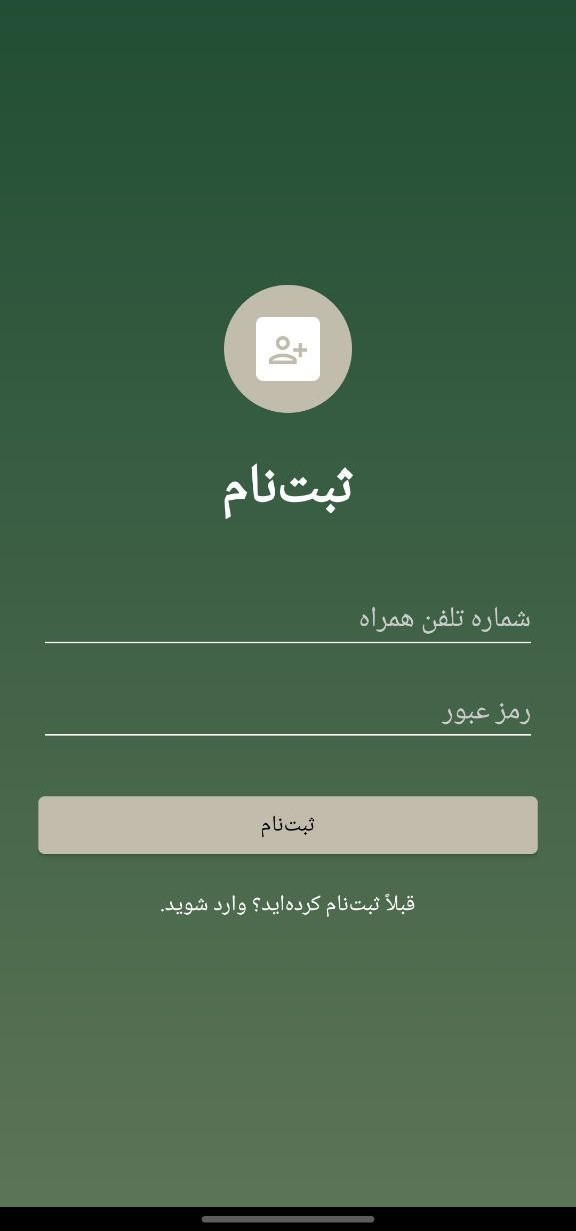
\includegraphics[width=0.7\textwidth,height=10cm,keepaspectratio]{Pic/signup}
		\caption{ورود/ثبت نام}
		\label{fig:auth}
	\end{subfigure}
	\begin{subfigure}[b]{0.3\textwidth}\centering
	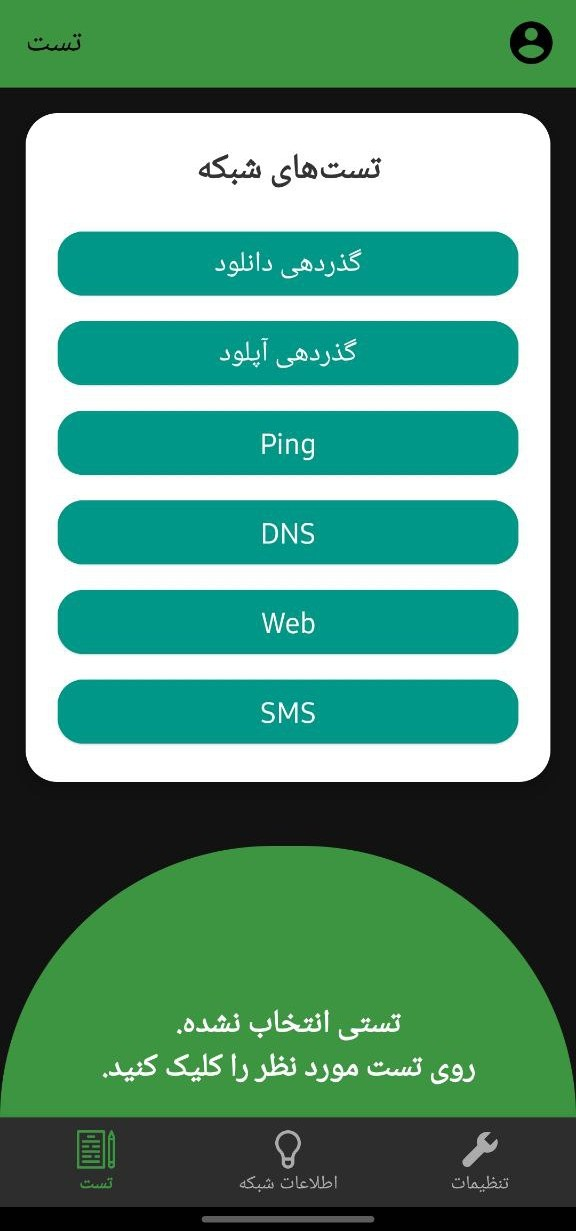
\includegraphics[width=0.7\textwidth,height=10cm,keepaspectratio]{Pic/test}
		\caption{تست ها}
		\label{fig:test}
	\end{subfigure}\\*[5mm]
	\begin{subfigure}[b]{0.3\textwidth}\centering
	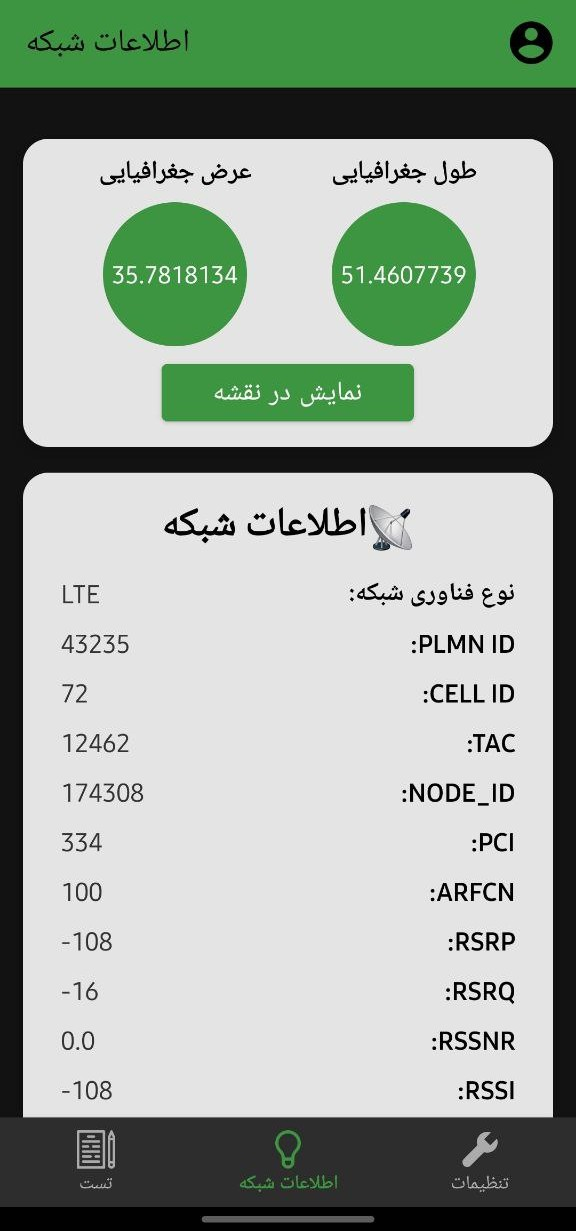
\includegraphics[width=0.7\textwidth,height=10cm,keepaspectratio]{Pic/info}
		\caption{اطلاعات}
		\label{fig:info}
	\end{subfigure}
	\begin{subfigure}[b]{0.3\textwidth}\centering
	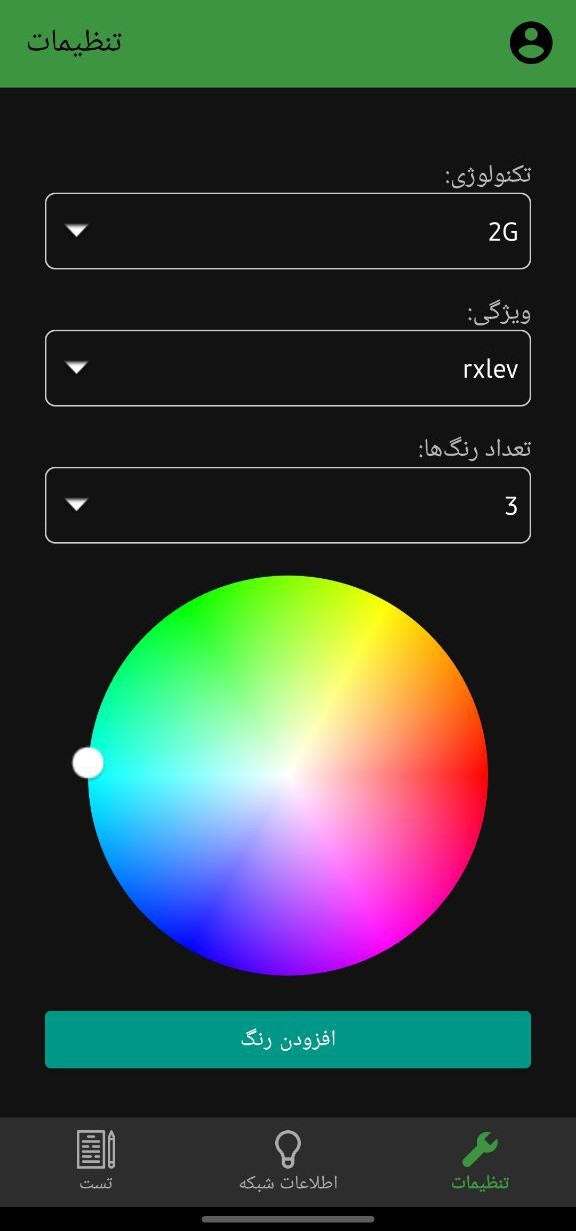
\includegraphics[width=0.7\textwidth,height=10cm,keepaspectratio]{Pic/setting}
		\caption{تنظیمات}
		\label{fig:setting}
	\end{subfigure}
	\begin{subfigure}[b]{0.3\textwidth}\centering
		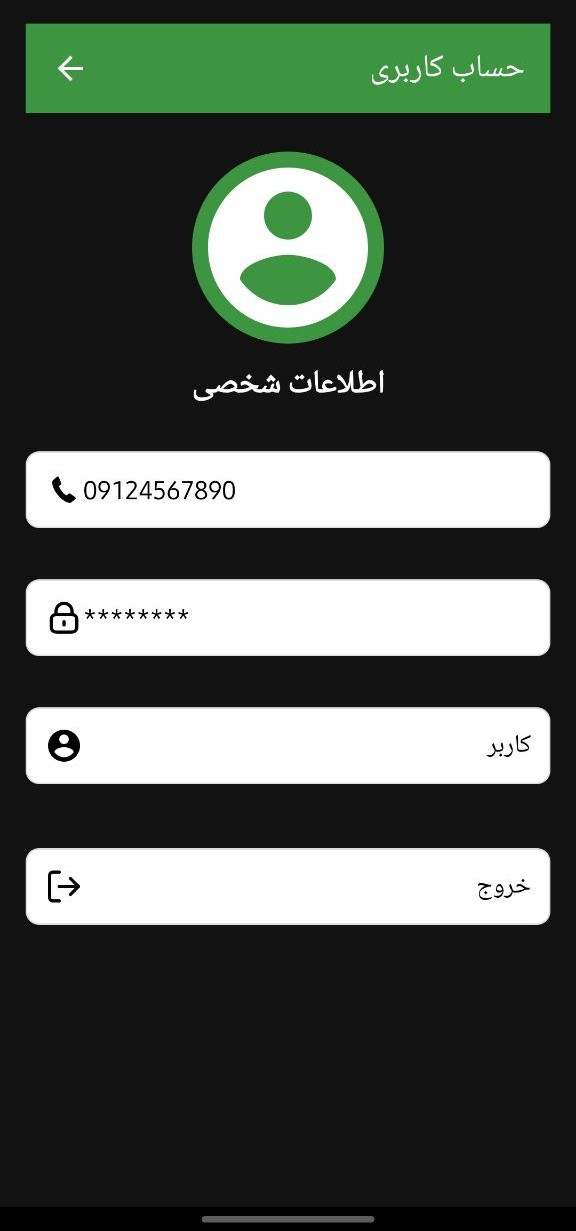
\includegraphics[width=0.7\textwidth,height=10cm,keepaspectratio]{Pic/profile}
		\caption{حساب کاربری}
		\label{fig:signup}
	\end{subfigure}
	\caption{تصاویر صفحات نام برده شده}
	\label{fig:androidPages}
\end{figure}


 
\end{document}



